\documentclass{article}
\usepackage{amsmath}
\usepackage[monospacemath,cmtt]{wrisym}
%%%%%%%%%%%%%%%%%%%%%%%%%%%%%%%%%%%%%%%%%%%%%%%%%%%%%%%%%%%%%%%%%
\usepackage{graphicx}
\usepackage{alltt}
\usepackage{hyperref}
\usepackage{url}
%%%%%%%%%%%%%%%%%%%%%%%%%%%%%%%%%%%%%%%%%%%%%%%%%%%%%%%%%%%%%%%%%

\newcommand{\Janson}[1]{{\fontfamily{pjn}\fontencoding{T1}%
\fontshape{n}\selectfont #1}}
\newcommand{\Palatino}[1]{{\fontfamily{ppl}\fontencoding{T1}%
\fontshape{n}\selectfont #1}}
\newcommand{\Garamond}[1]{{\fontfamily{pad}\fontencoding{T1}%
\fontshape{n}\selectfont #1}}
\newcommand{\Times}[1]{{\fontfamily{ptm}\fontencoding{T1}%
\fontshape{n}\selectfont #1}}
\newcommand{\Helvetica}[1]{{\fontfamily{phv}\fontencoding{T1}%
\fontshape{n}\selectfont #1}}
\newcommand{\Futura}[1]{{\fontfamily{pfu}\fontencoding{T1}%
\fontshape{n}\selectfont #1}}
\newcommand{\Optima}[1]{{\fontfamily{lop}\fontencoding{T1}%
\fontshape{n}\selectfont #1}}
\newcommand{\cmtt}{\texttt{MathCMTT}\xspace}
\newcommand{\mono}{\texttt{MathMono}\xspace}

\providecommand{\metafont}{\textsf{METAFONT}\xspace}
\newcommand{\teTeX}{\textsf{te\TeX}\xspace}
\newcommand{\MikTeX}{\textsf{Mik\TeX}\xspace}
\newcommand{\Math}{\textit{Mathematica}\xspace}
\renewcommand\appendix{\par
  \setcounter{section}{0}%
  \setcounter{subsection}{0}%
  %\gdef\thesection{\@Alph\c@section}
  \gdef\thesection{\hskip .5em}}
%%%%%%%%%%%%%%%%%%%%%%%%%%%%%%%%%%%%%%%%%%
\raggedbottom 
\begin{document} 

\title{
The \MathLogo{} Virtual Font Package\\
\MathLogo{} Fonts for \LaTeXe{}\\
Version 2.0\\
Including CMTT Fonts\\
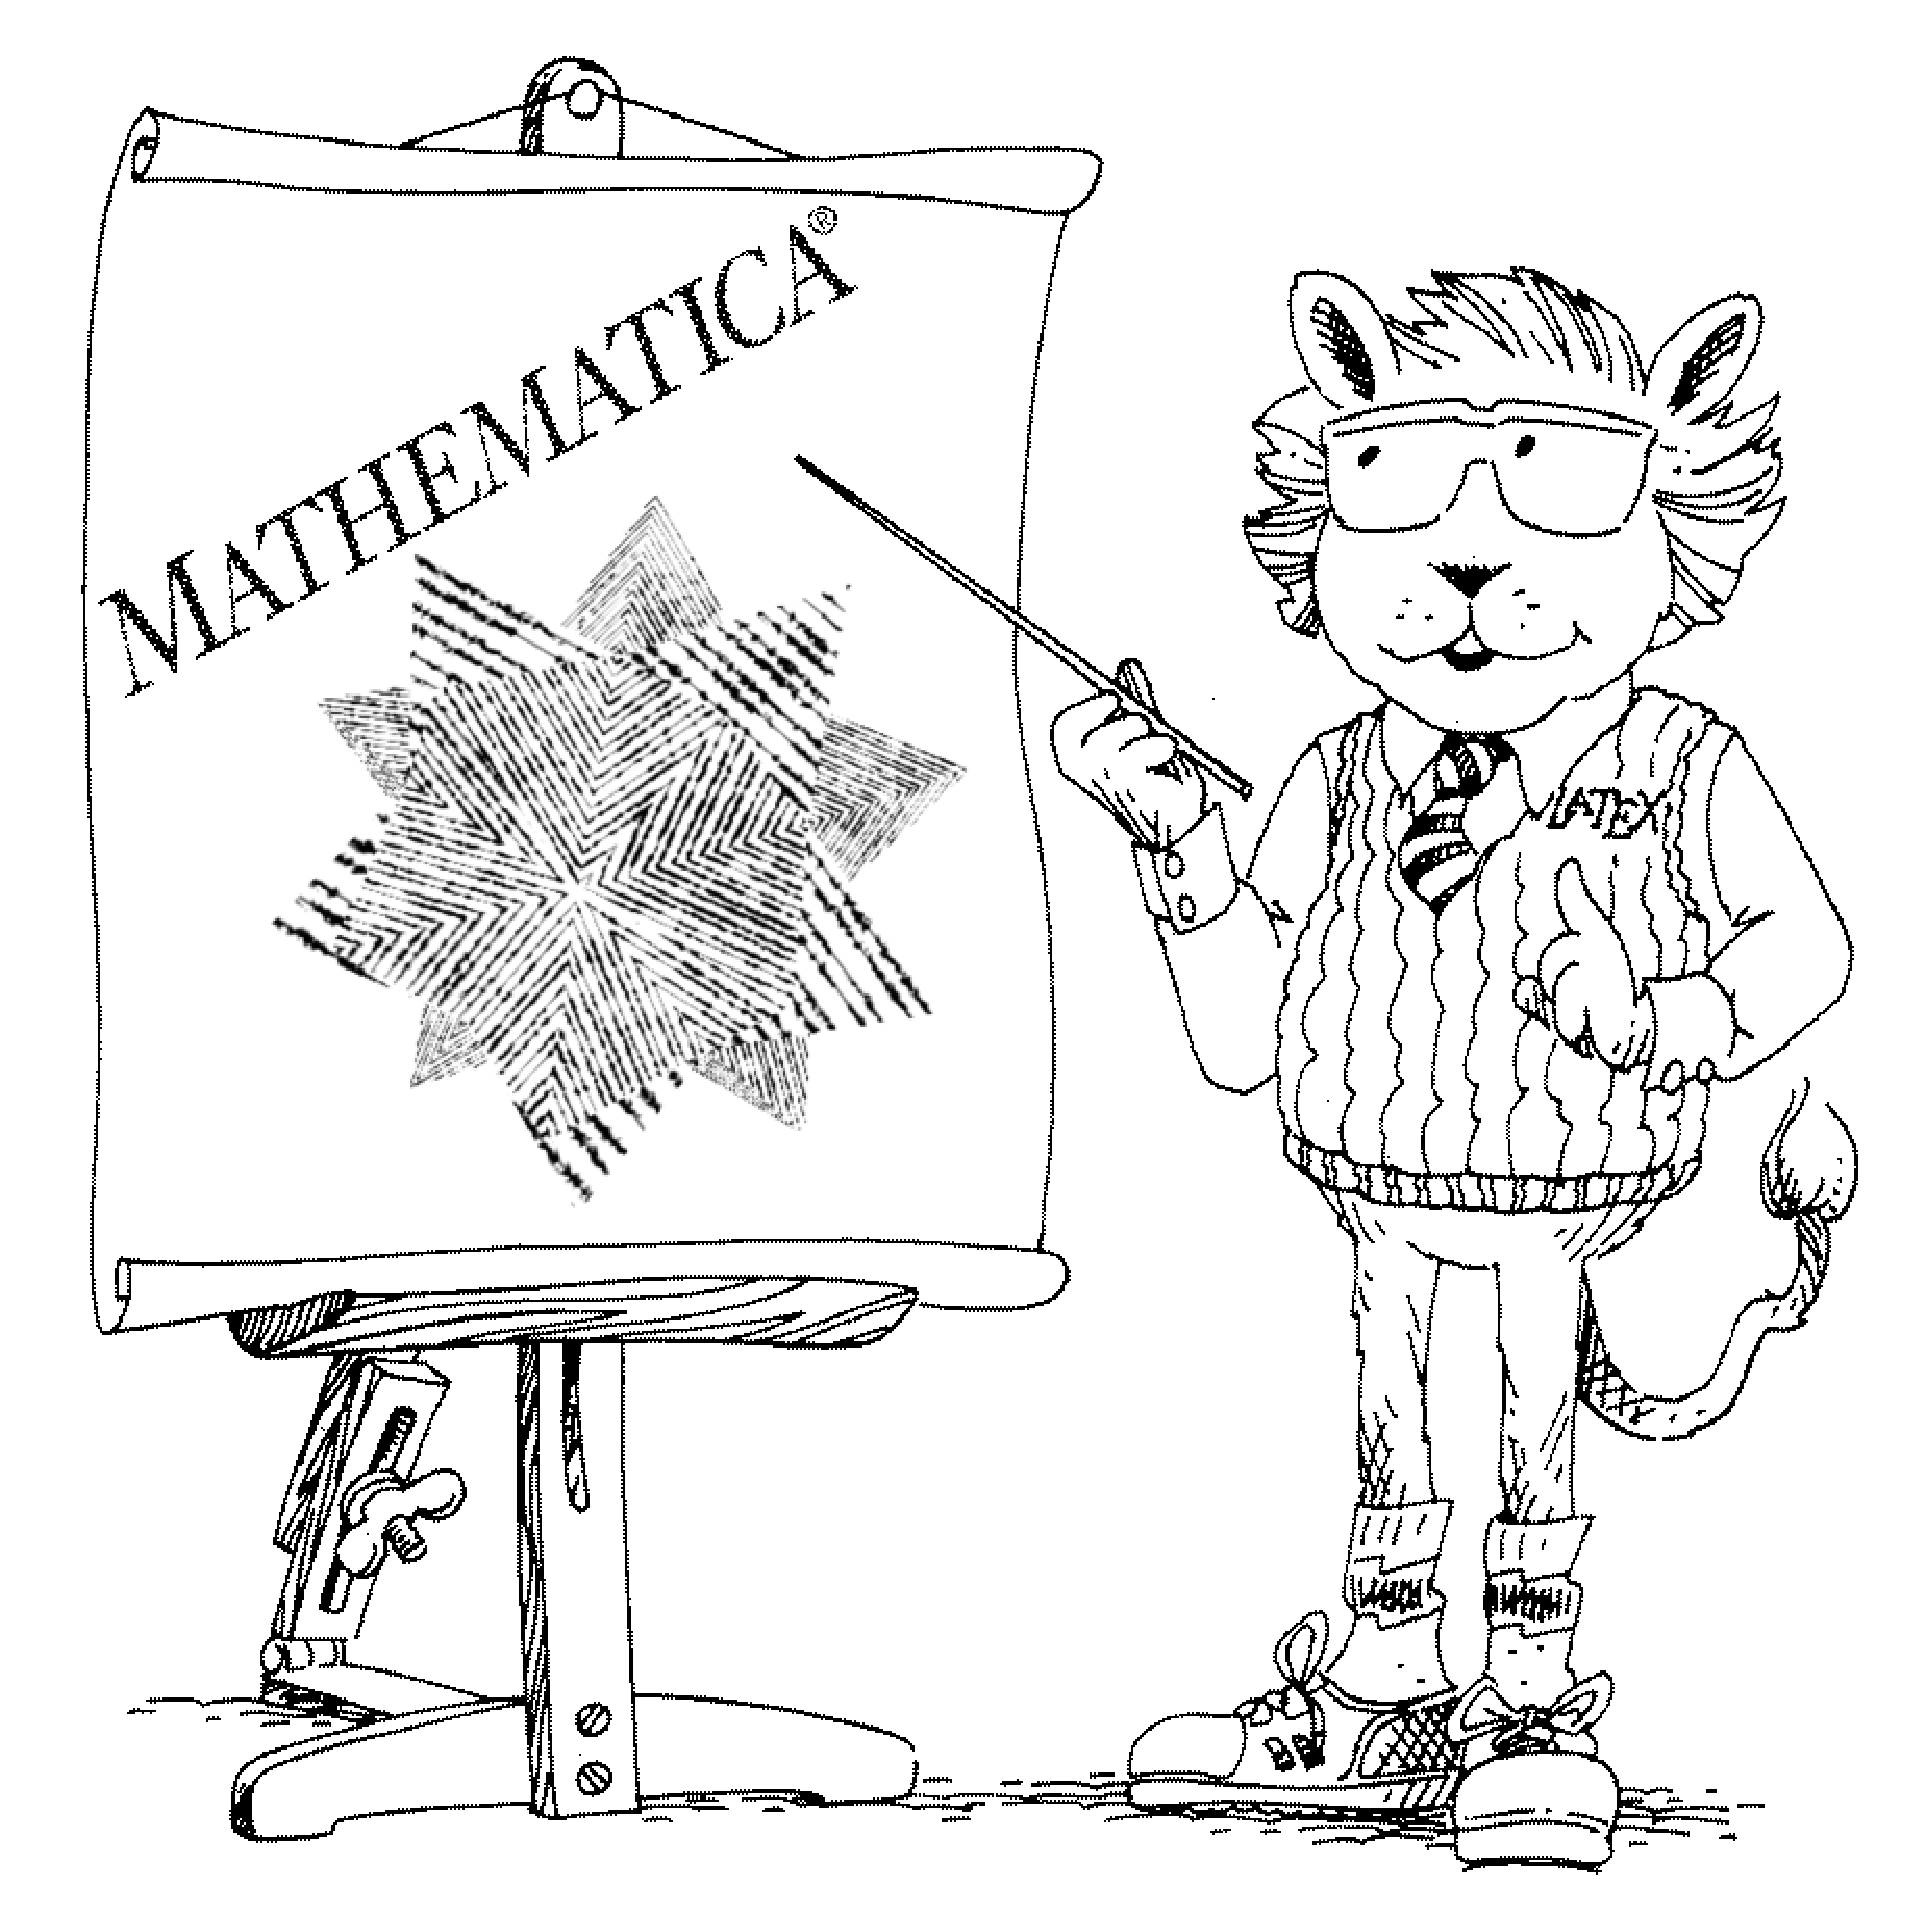
\includegraphics[width=0.8\textwidth]{fntpackcover}}
\date{May 2002}
\author{Jens-Peer Kuska}
\maketitle
\newpage
\tableofcontents
\newpage
\listoftables
\newpage
\section{Introduction}

\Math{} comes with a full set of mathematical fonts in PostScript
format. These fonts can be used to typeset mathematical texts in the
standard PostScript font, Times-Roman. To use the fonts with \TeX{}
and the macro package \LaTeXe{} \cite{LTeXComp}, you need more than
just the plain PostScript Type 1 fonts. \TeX{} must be given the
dimensions of the characters and, for typesetting mathematics, \TeX{}
needs the information on how to change the sizes of the operators and
delimiters coded in the fonts \cite{TeXBook}.

\TeX{} normally uses the Computer Modern fonts. These fonts are
generated by the \metafont program. \metafont produces bitmap fonts,
which are optimized for the resolution of the ouput device. These
bitmap fonts are included in the PostScript output as Type 3
fonts. When the PostScript file is printed on a device with a
different resolution, the bitmap fonts are scaled and the high quality
of the \metafont output is lost. Most PostScript fonts are
scalable-outline Type 1 fonts. The use of Type 1 fonts retains the
resolution independence of the PostScript file. \metafont cannot
create Type 1 fonts, but most modern \TeX{} distrubutions come with
Type 1 versions of the Computer Modern family.

Changing the text fonts to another font, like Times, produces a
PostScript output with mixed Type 1 fonts in text and Computer Modern
fonts in the mathematics mode.  Since Computer Modern does not fit
well with Times, you need mathematical fonts designed for use with
Times. These fonts are typically available commercially. The problem
is that \TeX{}'s mathematical fonts use characters from the fonts for
ordinary text. Operators, such as $\sin x$ and $\log z$, use the
operator font and the variables, like $x$, use the math-italic font. A
new text font also needs new versions of \TeX{}'s operator and
math-italic font, otherwise \textit{italic} and $italic$ use different
fonts.  To allow greater freedom of fonts for the text, the font
package includes fonts to use with \Times{Times}, \Janson{Janson}, and
\Garamond{Adobe Garamond}. For each base font, an operator and a
math-italic font are included. The first font is a standard PostScript
font, the next two are commercial fonts\footnote{To use the commercial
fonts, you have to buy the Type 1 fonts from
\href{http://www.adobe.com}{Adobe}.}.  \textit{The Mathematica
Journal} uses \Janson{Janson} as its text font and now the virtual
fonts are included to generate a similar layout. The new package
options \texttt{palatino}, \texttt{garamond}, and \texttt{janson}
select the new text, operator, and math-italic fonts.

Since \Math's input is traditionally typeset with monospaced
fonts, the typesetting of \Math sessions needs monospaced
mathematics fonts available only from the original \Math fonts.
Additionally the \Math fonts offer more symbols than the
traditional Computer Modern fonts. The symbols for natural, real, and
complex numbers ($\dsN$, $\dsR$, and $\dsC$) are included, as well as
path integrals, such as $\oint_\Gamma$, $f(z)$, $\dd z$, and surface
integrals.

\Math's Type 1 fonts cannot be used directly with \TeX.  There are
some basic differences between Type 1 fonts and \TeX{} fonts. The most
notable difference is that \TeX{} fonts include the information needed
for mathematical typesetting.  The \TeX{} metric files
(\textsf{*.tfm}) include information on how extensible symbols are
created from its pieces and how integral and sum signs are enlarged.
The virtual font package adds this information and offers a set of
macros to access the characters in the fonts.

A second monospaced font set called \cmtt is used to typeset
\textit{The \Math{} Book,} besides the fonts that come with the \Math{}
distribution.  These fonts are narrower than the usual Courier/\mono
combination. This makes the fonts ideal for typesetting the two-column
\texttt{In[]}/\texttt{Out[]} dialogs\footnote{ The font package itself
offers no macros to create such dialogs.  It contains only the
character definitions.}  in \textit{The Mathematica book.} In addition
to the mathematical symbols, the \cmtt fonts also replace the standard
typewriter font.  The new option \texttt{cmtt} allows the usage
of narrow \cmtt fonts.

\TeX{} provides the virtual font mechanism to allow you to borrow
characters from certain fonts and to assemble new ones.  \Math{}
has introduced some new symbols, such as $\ii=\sqrt{-1}$ and $\ee$ for
the base of the natural logarithm and the mathematical alphabets
$\mathbb{DoubleStruck}$, $\mathfrak{Gothic}$, and $\mathcal{Script}$
with lowercase letters. Similar mathematical alphabets can be found in
the font sets of the American Mathematical Society (AMS). The virtual
fonts, \textsf{w*.vf} and \textsf{w*.tfm}, and the style file,
\textsf{wrisym.sty}, replace the standard Computer Modern fonts.  The
four mathematical fonts for operators, letters, symbols, and
extensible symbols are replaced by the virtual fonts of the
\textsf{w*} family. The first 128 characters of the new fonts conform
to the standard \TeX{} encoding for mathematical fonts. Some of the
slots with higher character codes are used for the new symbols. The
main part of \textsf{wrisym.sty} deals with the setup of the new
symbols.

The standard options will use \Times{Times-Roman}{} and
\Helvetica{Helvetica}, the \texttt{garamond} option uses
\Garamond{Adobe Garamond} and \Optima{Optima}, and the \texttt{janson}
option uses \Janson{Janson} and \Futura{Futura} for text and
\textsf{sans serif text}. The sans serif font is not used by the
mathematical fonts and is only set to give a suggestion for the sans
serif font in the document.

The virtual fonts were created with Alan Jeffrey's fontinst package
\cite{GrComp}.

\begin{figure}
\includegraphics[width=0.5\textwidth]{MikTeXFntPack}
\caption{Add the path for the font package tree to the TDS root directories
of MikTeX.}\label{Fig::AddMikRoot}
\end{figure}

\begin{figure}
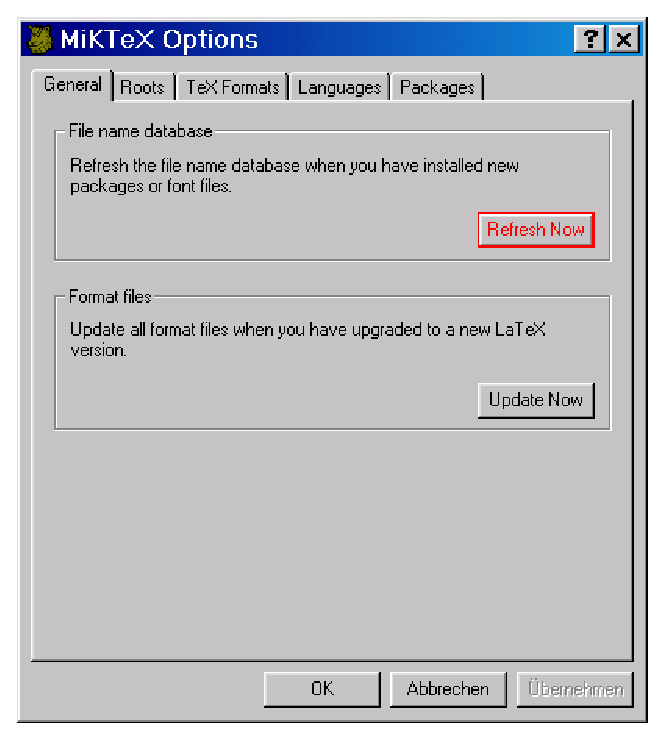
\includegraphics[width=0.5\textwidth]{MikTeXRefresh}
\caption{\hbox to \hsize{Refresh the file name data base.\hfill}}\label{Fig::MikRefresh}
\end{figure}


\section{Installation and Files}

All the files come in a single archive file with a TDS (\TeX{}
Directory Structure) conform structure.  \textsf{MikTeX} and \teTeX
support multiple root directories for the TDS tree. The best way to
install the font package is to unpack the archive file of the font
pack and to add the expanded tree to the TDS root directories searched
by your \TeX{} installation.


\subsection{\MikTeX on a Windows System}
\begin{sloppypar}
Expand the archive in a folder like \textsf{MathematicaFontPack}.
Open the \MikTeX $|$ \MikTeX Options program, choose the \textsf{Roots}
section, and add the directory \textsf{MathematicaFontPack$\backslash$texmf}
to the root directories (see \figurename{} \ref{Fig::AddMikRoot}).
Refresh the file name database (see \figurename{} \ref{Fig::MikRefresh}).
Modify the \textsf{config.ps} file and the \textsf{pdftex.cfg} 
by adding the map files.
For \textsf{config.ps} the section for the PostScript font mapping 
should look like this:
\end{sloppypar}
\begin{verbatim}
% An "all-in-one" psfonts.map.
p psfonts.map
% and the LaserWriter 35 fonts *not* in Acrobat. pdftex loads
% these differently
p +lw35extra.mapfile
p +wolfram.map
\end{verbatim}

\noindent{}The \textsf{config.ps} file should be in the 
\textsf{texmf$\backslash$dvips$\backslash$config}
directory.
The configuration  \textsf{pdftex.cfg} for 
\textsf{pdftex} must also be changed and should 
look like this:
\begin{verbatim}
pk_resolution 600
output_format 1
compress_level 9
decimal_digits 3
page_width 210 true mm
page_height 297 true mm
horigin 1 true in
vorigin 1 true in
map psfonts.map
map +pdfwolfram.map
\end{verbatim}

\noindent{}The configuration file should be in
\textsf{texmf$\backslash$pdftex$\backslash$config}.  Now this document
should compile with \LaTeX{} and \textsf{pdflatex}.

For \textsf{fpTeX} on a Windows system, the instructions for \teTeX
should be used.


\subsection{\teTeX on a Unix System}

\teTeX also allows multiple TDS root directories. If the font package
archive is expanded in \textsf{/usr/local/tex/MathematicaFontPack},
the new TDS root must be added to the \textsf{texmf.cfg} file. This
file can be found in the \textsf{\$TEXMF/texmf/web2c} directory. At
the begin of the file the \texttt{TEXMF} variable is set. This part of
the \textsf{texmf.cfg} file should changed to look like this:
\begin{verbatim}
% Now, list all the texmf trees. If you have multiple trees,
% use shell brace notation, like this:
%   TEXMF = {$HOMETEXMF,!!$VARTEXMF,!!$TEXMFLOCAL,!!$TEXMFMAIN}
% The braces are necessary.
%
% A place to store other TeX support files. Can be a remote
% texmf tree, or a tree to store non-free stuff, or ...
%   TEXMFEXTRA=$SELFAUTOPARENT/texmf-extra
% If you set this, add $TEXMFEXTRA in the list below
%
% Define the tree with the font pack
WRITREE=/usr/local/tex/MathematicaFontPack/texmf
%
% Add the new TDS root to the TEXMF variable
TEXMF = {$HOMETEXMF,!!$WRITREE,$TEXMFLOCAL,!!$TEXMFMAIN}
\end{verbatim}
Now the filename data base must be updated by a \texttt{texhash} or
\texttt{texconfig rehash} command from the shell.

\teTeX programs use the first configuration file in the TDS tree
list. The font package comes with configuration files and, if you
choose another position on the font package tree in the list
\texttt{TEXMF}, you must add the map files in the configuration of
\textsf{dvips} and \textsf{pdftex} in the TDS root that is scanned
first.


\subsection{Words of Caution}

When the font package is used with
\href{http://www.miktex.org}{\MikTeX} or with
\href{http://www.tug.org/texlive}{TeXLive} some care must be taken to
get a working installation.

The map files in the font pack also include the correct declarations
of the old fonts. This may be a useful way to include figures
generated by \Math 3.0--4.1 into \TeX{} documents.

Both distributions come with a \textsf{psfonts.map} file that already
includes the old \Math{} fonts. The map file in the TeXLive
distribution uses lowercase characters for the font names. Since Unix
file names are case sensitive, a TeXLive installation will not find
the \Math{} fonts because the \textsf{psfonts.map} include lines
like this:
\begin{alltt}
Math1 Math1 <math1.pfb
\(\vdots\)
\end{alltt}
%
All references to the mistyped font names must be removed from the
\textsf{psfonts.map}, and the correct map file from the \Math{}
virtual font distribution must be added as described above.  To remove
the false entries from the map file, you need root access to the
\TeX{} installation.

The case errors in the \textsf{psfonts.map} file that comes with
\MikTeX should have no effect, but it turns out that the multiple
definitions of the font files in the \MikTeX configuration and in the
\textsf{wolfram.map} file create errors when \MikTeX searches the
fonts. All references to the \Math{} fonts must be removed from
the \textsf{psfonts.map} that come with \MikTeX.

This also applies to the \textsf{psfonts.map} file for
\textsf{pdftex}.  This file is in the configuration directory of
\textsf{pdftex}.
\begin{sloppypar}
The \MikTeX distribution and the \teTeX distribution come with a file
\textsf{fontname/wolfram.map}. This file includes references to the
virtual fonts createt by Ulrik Vieth. These fonts are incomplete and
the name of the map file will prevent the inclusion of the
\textsf{wolfram.map} file that comes with the virtual font package.
\emph{This file must be deleted!}
\end{sloppypar}


\subsection{More Details}

To use the fonts, a DVI-driver that understands virtual fonts like
\textsf{dvips}\footnote{\textsf{dviwindo} from Y\&Y and the PC\TeX{}
driver do not support virtual fonts.} is needed. The common screen
drivers, such as \textsf{xdvi} from
\teTeX\footnote{\url{www.tug.org/tetex/}} and fp\TeX{} or
\textsf{yap} from \href{http://www.miktex.org}{\MikTeX}\!, support
virtual fonts.

The new fonts all start with the letter \textsf{w} for Wolfram
Research.  The combination with \Times{Times} is indicated by the
letters \textsf{tm}, \Janson{Janson} by the letters \textsf{jn},
\Garamond{Garamond} by \textsf{ad}, the monospaced fonts with Courier
by the letters \textsf{cr}, and the \cmtt monospaced fonts by
\textsf{tt}.  The fourth letter corresponds to the font type:
\texttt{r} for regular OT1 fonts, \texttt{m} for OML, \texttt{y} for
OMS, or \texttt{v} for OMX. If the fifth letter is a \texttt{u}, it is
the upright math-italic font. The final letter stands for the weight
of the font: \texttt{m} for medium and \texttt{b} for bold. Therefore,
the font \textsf{wttvm} is the \cmtt\ font in OMX encoding with a
medium weight.

\begin{table}
\caption[Metric files in the distribution]{Metric files in the distribution.}
\begin{center}
\begin{tabular}{|rll | c | l|}
\hline\hline
\textsf{wtm}&\textsf{r}&\textsf{m$\vert$b} & OT1 & \Times{Times} operator\\
\textsf{wtm}&\textsf{m}&\textsf{m$\vert$b} & OML & \Times{Times} math italic\\
\textsf{wtm}&\textsf{y}&\textsf{m$\vert$b} & OMS & \Times{Times} symbol\\
\textsf{wtm}&\textsf{v}&\textsf{m$\vert$b} & OMX & \Times{Times} math extensions\\
\hline
\textsf{wjn}&\textsf{r}&\textsf{m$\vert$b} & OT1 & \Janson{Janson} operator\\
\textsf{wjn}&\textsf{m}&\textsf{m$\vert$b} & OML & \Janson{Janson} math italic\\
\hline
\textsf{wad}&\textsf{r}&\textsf{m$\vert$b} & OT1 & \Garamond{Garamond} operator\\
\textsf{wad}&\textsf{m}&\textsf{m$\vert$b} & OML & \Garamond{Garamond} math italic\\
\hline
\textsf{wcr}&\textsf{r}&\textsf{m$\vert$b} & OT1 & Courier operator\\
\textsf{wcr}&\textsf{m}&\textsf{m$\vert$b} & OML & Courier math italic\\
\textsf{wcr}&\textsf{y}&\textsf{m$\vert$b} & OMS & Courier symbol\\
\textsf{wcr}&\textsf{v}&\textsf{m$\vert$b} & OMX & Courier math extensions\\
\textsf{wcru}&\textsf{m}&\textsf{m$\vert$b} & OML & Courier math italic upright\\
\hline
\textsf{wtt}&\textsf{r}&\textsf{m$\vert$b} & OT1 & \cmtt operator\\
\textsf{wtt}&\textsf{m}&\textsf{m$\vert$b} & OML & \cmtt  math italic\\
\textsf{wtt}&\textsf{y}&\textsf{m$\vert$b} & OMS & \cmtt  symbol\\
\textsf{wtt}&\textsf{v}&\textsf{m$\vert$b} & OMX & \cmtt  math extensions\\
\textsf{wttu}&\textsf{m}&\textsf{mv} & OML & \cmtt math italic upright\\
\hline
\textsf{wsb} & & \textsf{m$\vert$b}  &  U  &  Keyboard and text symbols \\
\hline
\textsf{wtt} & & \textsf{r8t}         & T1 &  \cmtt  text font\\
\textsf{wtt} & & \textsf{ro8t}         & T1 &  \cmtt  italic text font\\
\textsf{wtt} & & \textsf{b8t}         & T1 &  \cmtt  text font\\
\textsf{wtt} & & \textsf{bo8t}         & T1 &  \cmtt italic text font\\
\hline
\end{tabular}
\end{center}
\end{table}

\begin{sloppypar}
\TeX{} needs the font metric files (\textsf{*.tfm}), the virtual fonts
(\textsf{*.vf}), and the native font metric files from the \Math{}
fonts (i{.}e{.}, \textsf{Mathematica1.tfm}, \textsf{Mathematica2.tfm},
\ldots).  \LaTeXe{} needs the font definition files
\textsf{OT1w*r.fd}, \textsf{OMLw*m.fd}, \textsf{OMSw*y.fd}, and
\textsf{OMXw*v.fd} to access the fonts. Additionally, the font
definitions for the Times-Roman (\textsf{T1ptm.fd}), Helvetica
(\textsf{T1phv.fd}), Courier fonts (\textsf{T1pcr.fd}), and \cmtt
(\textsf{T1wtt.fd}) are needed for the style file
\textsf{wrisym.sty}. The first three files usually come with the
\LaTeXe{} packages in the \textsf{psnfss} directory.  If you need to
combine with other fonts, such as \Janson{Janson} or
\Garamond{Garamond}, the metric files and virtual fonts are included
in the corresponding parts of the directory tree.  The commercial
fonts (\texttt{*.pfb}) are not included and must be obained from the
font vendors.
\end{sloppypar}

A DVI driver creating PostScript output must be told to download the
Type 1 \Math{} fonts.  A typical line in this map file looks like
this:
\begin{alltt}
Mathematica1 Mathematica1 <Mathematica1.pfa
\(\vdots\)
\end{alltt}

This map file includes the \Math{} fonts in your PostScript
output.  This is useful when the document needs to be printed on a
system that does not have the \Math fonts installed. To reduce the
file size, the driver should be forced to reencode the fonts. This
removes unused glyphs from the fonts. For \textsf{dvips} and
\textsf{pdftex} the reencoding is forced with the \texttt{-j0} option.

Leaving the fonts out of the PostScript file will minimize the file
size.  The PostScript file then contains references to the appropriate
\Math{} fonts instead of the fonts themselves.  However, only
those who already have the \Math{} fonts available to their
resident PostScript interpreter (a PostScript interpreter might be a
copy of Ghostscript, a PostScript printer, or some other PostScript
rasterizing system) will be able to correctly view your PostScript
file. This behavior can be achieved by removing the last row in the
map file, the lines should look like this:
\begin{alltt}
Mathematica1 Mathematica1 
\(\vdots\)
\end{alltt}


\subsection{Using Ghostscript}

To setup the fonts for Ghostscript, Ghostscript must be told where the
fonts can be found.  This is usually done by setting/appending the
directory with the \Math{} fonts (usually
\textsf{/usr/local/mathematica/SystemFiles/Fonts/Type1}) to the
\verb|GS_LIB| environment variable in your login shell script.

Windows users can set the \verb|GS_LIB| variable in the
\textsf{autoexec.bat} file or in the advanced options of
\textsf{GSView} (see \figurename{} \ref{Fig::GSPath}).

\begin{figure}
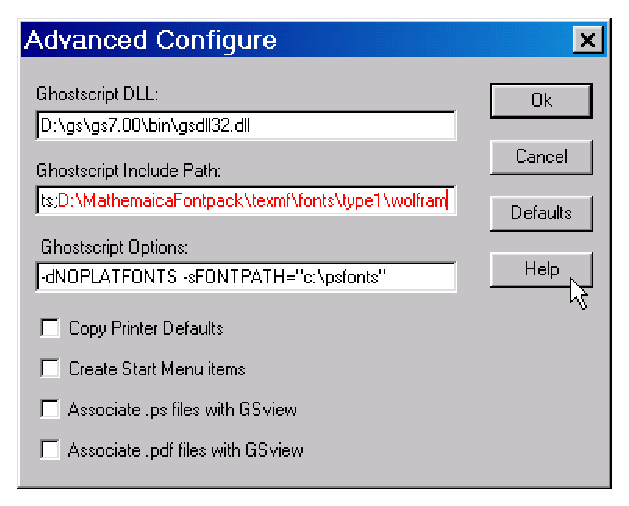
\includegraphics[width=0.5\textwidth]{GSPath}
\caption{\hbox to \hsize{Set the search path for Ghostscript in GSView.\hfill}}\label{Fig::GSPath}
\end{figure}


\section{Using Fonts with \LaTeXe}
To use the package with your own files add the line
\begin{verbatim}
\usepackage{wrisym}
\end{verbatim}
%
to the preamble of your \LaTeXe{} document.

If you get the font package from a \Math{} installation, you
should copy the Type 1 fonts from \Math's directory tree into a
directory \textsf{fonts/type1/wolfram} in your local \textsf{texmf}
tree. Than your \TeX{} installation is independent of the \Math
installation and you will be able to translate your \TeX{} sources
even when \Math{} is uninstalled or the installation directory is
changed.

The style file has several options. It automatically loads the font
encoding package and switches to the T1 encoding.  The possible
options for the package are:
\begin{description}
\item[{\normalfont\texttt{times}}]  load the fonts with \Times{Times} as base font.
      This is the default setting and should work with any PostScript
      printer. No additional fonts are needed.

\item[{\normalfont\texttt{janson}}] load the fonts with \Janson{Janson} as base font.
      The Janson fonts from Adobe must be available to use this option.
      
\item[{\normalfont\texttt{garamond}}] load the fonts with \Garamond{Adobe Garamond} as 
      base font. The Garamond fonts from Adobe must be available to use 
      this option.

\item[{\normalfont\texttt{monospacemath}}] declare the mathematics versions for
      monospaced mathematics like 
      \mathversion{mono}$\int_0^\infty \psi^*(r)\psi(r) r^2 \dd r$.   
      \mathversion{normal} These fonts are not loaded by
      default.
      
\item[{\normalfont\texttt{cmtt}}] use the \cmtt fonts for monospaced mathematics.      
     This option also implies the \texttt{monospacemath}
     option.
\item[{\normalfont\texttt{uprightmonomath}}] use upright letters instead of italic
    letters in monospaced mathematics. This option also implies 
     the \texttt{monospacemath} option.
\end{description}


Apart from the production of bitmap-free \TeX{} output, you may use
monospaced mathematical fonts. This is of limited interest in ordinary
mathematical texts, but it is needed for typesetting the \texttt{In[]}
and \texttt{Out[]} cells of \Math{} notebooks.  For this purpose
\textsf{wrisym.sty} introduces two new mathematical styles.  The
\textsf{wrisym.sty} package has an option \texttt{monospacemath}.  If
the package is loaded with

\begin{verbatim}
\usepackage[monospacemath]{wrisym}
\end{verbatim}

\noindent{}then the monospaced fonts will be present and two new math
versions are defined.  For medium weight monospaced output, the
math-style \texttt{mono} is introduced, and for bold monospaced
mathematics, the \texttt{monobold} is introduced.  By default the
monospaced fonts will not be loaded.
\begin{sloppypar}
Like the \texcmd{boldmath} or \verb|\mathversion{bold}| (\figurename{}
\ref{Fig:mathbold}), the commands \texcmd{monomath} or
\verb|\mathversion{mono}| ((\figurename{} \ref{Fig:mathmono}) and
\texcmd{monoboldmath} or \verb|\mathversion{monobold}| (\figurename{}
\ref{Fig:mathmonobold}) will switch to the new styles. Remember that
the switch must be outside of a mathematical formula.  The command
\verb|\mathversion{normal}| (\figurename{} \ref{Fig:mathnormal}) will
restore the default font set.  Typesetting notebooks will require many
more macros than \textsf{wrisym.sty} introduces.
\end{sloppypar}

\def\half{\frac{1}{2}}

\def\mathsample{\fbox{\begin{minipage}{0.975\textwidth}
\noindent The Dirac equation for a free particle:
\[ \ii \hbar \frac{\partial \psi}{
              \partial t} = {\hat H}_f \psi = 
	\left( \dsc\, {\hat{\vec \alpha}}\,{\hat{\vec p}} + m_0\, \dsc^2\, {\hat \beta}\right)\psi
\]
\noindent
The integral representation of Bessel function $J_\nu(z)$ :
\begin{eqnarray}
J_\nu(z)&=&\frac{1}{\pi}
              \int_0^\pi \cos( z \sin(\theta)-\nu\,\theta)\,\dd\theta\nonumber\\%
		  &&\qquad-
		  \frac{\sin(\nu\pi)}{
		   \pi} \int_0^{\infty} \ee^{z \sinh t - \nu\,t}\,\dd t
		   \,\, (|\arg z|<\frac{1}{2}\pi)\nonumber
\end{eqnarray}
The expansion of Coulomb wave functions in terms of Bessel-Clifford functions:
\[
F_L(\eta,\varrho)=C_L(\eta) \frac{(2\,L+1)!}{
                             (2\,\eta)^{2\,L+1}} \varrho^{-L} 
							 \sum_{k=2\,L+1}^\infty b_k t^{k/2} I_k(2\sqrt{t})
\]
with $b_{2\,L+1}=1$, $b_{2\,L+2}=0$ and 
$4\eta^2\,(k-2\,L)\,b_{k+1}+k\,b_{k-1} + b_{k-2}=0$.

\vskip\baselineskip

\noindent A radical identity:
\[
\sqrt{\half}\cdot\sqrt{\half+\half\,\sqrt{\half}}\cdot
\sqrt{
  \half +\half\sqrt{
    \half+\half\sqrt{\half}
   }
 }\ldots = \frac{2}{\pi}	
\]
\begin{equation}\begin{split}
   p(R,\phi,\theta)\sim&
   \rho\omega^2
   e^{-\imath\pi/4} \sqrt{\frac{a}{2 \pi^3 R\cos\phi}}
   \sum_{n=0}^{\infty} (-\imath)^n \cos(n\theta) \\
   &\times
   \left \{   
   \int_{-\infty}^{\infty} 
        \frac{\tilde{W}_n(\gamma)
              \exp\left[\imath R/a 
                   \left(
                     \sqrt{k^2 a^2 -\gamma^2} \cos\phi
                     + \gamma\sin\phi
                   \right)
                  \right]}
             {\left(k^2 a^2 -\gamma^2 \right)^{3/4}
              {{H}_n^{\mbox{\tiny $(1)$}}}' 
           \left(\sqrt{k^2 a^2 -\gamma^2}\right)}
      \;d\gamma
    \right \}
\end{split}\end{equation}
\end{minipage}
}
}

\begin{figure}
\mathsample
\caption{The normal mathematics style.}\label{Fig:mathnormal}
\end{figure}

\begin{figure}
\boldmath\mathsample
\caption{The bold mathematics style.}\label{Fig:mathbold}
\end{figure}

\begin{figure}
\monomath\mathsample
\caption{The mono mathematics style.}\label{Fig:mathmono}
\end{figure}

\begin{figure}
\monoboldmath\mathsample
\caption{The mono bold mathematics style.}\label{Fig:mathmonobold}
\end{figure}
\mathversion{normal}

\begin{sloppypar}
One difference between the monospaced output and the fonts used for
\textit{The Mathematica Book} is that the variables are typeset in
italics.  This is the correct behavior for mathematics, but it looks
strange for constructs like
\mathversion{mono}$$Expand[(x^2+1)^{100}]$$\mathversion{normal}
\end{sloppypar}

The package also provides monospaced 
math-italic fonts with upright characters. 
The upright monospaced characters are loaded with the 
package option \texttt{uprightmonomath}.

When the narrower version of the monospaced fonts should be used to
typeset a \Math{} session, the \texttt{cmtt} option should be given to
the package. The \texttt{cmtt} option will define the monospaced
mathematics styles.


\section{Symbol Names}

The \Math{} names, in most cases, are too long. The \TeX{} command
for a symbol is the name of the corresponding AMS font symbol, if it
exists, otherwise a \Math{} alias or name is used.  Negated
relations always start with the letter \texttt{n} and the \TeX{} or
AMS-\TeX{} name follows. Even if it is not explicitly listed in the
following tables, an alias in the \Math{} naming convention
may exist.

\begin{sloppypar}
The additional alphabets all work with the full \Math{} name; the
aliases of the frontend; and the AMS font switching mechanism using
\verb|\mathcal{}| for script, \verb|\mathfrak{}| for \Math{}s
gothic, and \verb|\mathbb{}| for double-struck characters. For single
letters, you should use the alias of the front end because the macros
for character replacement in the \verb|\mathcal{}|, \verb|mathbb{}|,
and \verb|\mathfrak{}| commands are a bit time consuming.
\end{sloppypar}


\section{Changes}
Since the 1.0 release, I have fixed some bugs in the italic correction
of the greek characters and the font dimension parameters. My thanks
go to Ulrik Vieth and Jaiyong Lee (\verb|jai@arctic.mit.edu|) for the
bug reports.

Version 2.0 adds the support for \textsf{pdftex}, the options to use
the \cmtt fonts, and the combinations with \Janson{Janson} and
\Garamond{Adobe Garamond}. Since the new \Math{} fonts include some
more glyphs, these new characters and symbols are added to the fonts
and to the style file. The most important additions are double-struck
digits and the symbols for Euro currency (\euro) and logical
operations.


\section{Bug Reports}

I have still some free positions in the virtual fonts. All users are
asked to contribute requests for PostScript font symbols that are
missed in the \TeX{} fonts.

The virtual fonts (spacing, italic correction, placement of super- and
subscripts, and so on) as well as the style file, \texttt{wrisym.sty},
may still have some errors. Please report any bugs via email to:

\begin{quote}
\href{kuska@informatik.uni-leipzig.de}{kuska@informatik.uni-leipzig.de}\\
\href{fontpack@wolfram.com}{fontpack@wolfram.com}
\end{quote}

Please start the subject line with ``\verb|Mathematica Font Bug|'' and
attatch a \LaTeXe{} file that shows the error. I will try to fix any
errors as soon as posible.


\section{Copyright}

% NOTE: Insert Standard WRI Font license language

Wolfram Research, Inc. reserves the right to control all distribution
of the \Math fonts and does not, at this time, allow them to be
widely distributed via any servers, archives, or non-Wolfram Research
software products of any kind without their express written
consent. There are no restrictions on embedding the fonts in documents
transmitted to service bureaus, publishers, or other users of Wolfram
Research products. There are no restrictions on widely distributing
metrics files generated from the \Math{} fonts.

The copyright of all files in the ``\Math{} Virtual Font Package''
belongs to Jens-Peer Kuska.

The files may be freely copied, distributed, and used, provided
no changes whatsoever are made.  All users are asked to help keep the
virtual font files and the style consistent and ``uncorrupted,'' so
they remain identical everywhere in the world.  Changes are
permissible only if the modified file is given a new name, different
from the names of existing files, and only if the modified file is
clearly identified as not being part of the ``\Math{} Virtual Font
Package''.
    
Every effort has been made to produce correct and useful macros and
fonts, in order to help promote computer science research and
\Math, but no warranty of any kind should be assumed.

\section*{Acknowledgments}

Andr{\' e} Kuzniarek, Gregg Snyder, and Stephen Wolfram made the
original font design. Andy Hunt prepared the Version 2.0 PostScript
fonts and fine tuned the fonts for use with the new set of virtual
fonts.  Many thanks go to \href{http://www.wolfram.com}{Wolfram
Research} for the creation of this set of mathematical PostScript
fonts.

The cover picture of the manual is a modified picture from Duane Bibby
from the \LaTeX{} manual.


\begin{thebibliography}{9}
\bibitem{GrComp} Michel Gossens, Sebastian Rahtz, and Frank Mittlebach,
                 \textit{The \LaTeX{} Graphics Companion}, Reading, Massachusetts, Addison-Wesley, 1997.
\bibitem{LTeXComp} Michel Gossens, Frank Mittlebach, and Alexander Samarin,
                 \textit{The \LaTeX{} Companion}, Reading, Massachusetts, Addison-Wesley, 1994.
\bibitem{TeXBook} Donald E. Knuth, \textit{The \TeX{}book}, Reading, Massachusetts, Addison-Wesley, 1984.
\end{thebibliography}
\appendix


%\section{\hskip -1em Appendix: Character Tables}
\section{\hskip -1.5em Appendix: Character Tables}

The following tables give the references for the defined characters and
symbols when the \textsf{wrisym.sty} package is used.

\def\charrow#1#2#3{\texcmd{#1} & \texcmd{#2} & $#3$ & {\boldmath $#3$}\\}

\begin{table}
\caption[Additional characters]{Additional characters.}
\begin{center}
\begin{tabular}{|c|c|c|c|}
\hline
Name & Alias & Normal & Bold \\
\hline
\charrow{ee}{ExponetialE}{\ee}
\charrow{ii}{ComplexI}{\ii}
\charrow{jj}{ComplexJ}{\jj}
\charrow{dd}{DifferentialD}{\dd}
\charrow{DD}{CapitalDifferentialD}{\DD}
\charrow{DoublePi}{}{\DoublePi}
\charrow{EulerGamma}{}{\EulerGamma}
\charrow{ScriptDotlessI}{}{\ScriptDotlessI}
\charrow{ScriptDotlessJ}{}{\ScriptDotlessJ}
\hline
\charrow{HBar}{hbar}{\hbar}
\charrow{Mho}{}{\Mho}
\charrow{lambdaslash}{}{\lambdaslash}
\charrow{Angstroem}{}{\Angstroem}
\hline
\charrow{beth}{}{\beth}
\charrow{daleth}{}{\daleth}
\charrow{gimel}{}{\gimel}
\hline
\charrow{Digamma}{}{\Digamma}
\charrow{Stigma}{}{\Stigma}
\charrow{Koppa}{}{\Koppa}
\charrow{Sampi}{}{\Sampi}
\charrow{digamma}{}{\digamma}
\charrow{stigma}{}{\stigma}
\charrow{koppa}{}{\koppa}
\charrow{sampi}{}{\sampi}
\charrow{varkappa}{}{\varkappa}
\charrow{Euler}{euler}{\Euler}
\charrow{Micro}{}{\Micro}
\hline
\end{tabular}
\end{center}
\end{table}

\def\SDCharRow#1#2#3#4{\texcmd{#1} & \texcmd{#2} &
                 $\csname #2\endcsname$  
				 &\texcmd{#3} & \texcmd{#4} &
                 $\csname #4\endcsname$ \\}

\def\DCharRow#1#2#3#4{\texcmd{#1} & \texcmd{#2} &
                 $\csname #2\endcsname$ 
				 & {\boldmath $\csname #1\endcsname$} 
				 &\texcmd{#3} & \texcmd{#4} &
                 $\csname #4\endcsname$ 
				 & {\boldmath $\csname #3\endcsname$}\\}
\begin{table}
\caption[Script characters]{Script characters. You can use
\texcmd{mathcal} to get 
several $\mathcal{Script}$ characters and digits $\mathcal{0123456789}$.}
\begin{center}
\begin{tabular}{|c|c|c|c|c|c|}
\hline
\SDCharRow{ScriptZero}{scZero}{ScriptOne}{scOne}
\SDCharRow{ScriptTwo}{scTwo}{ScriptThree}{scThree}
\SDCharRow{ScriptFour}{scFour}{ScriptFive}{scFive}
\SDCharRow{ScriptSix}{scSix}{ScriptSeven}{scSeven}
\SDCharRow{ScriptEight}{scEight}{ScriptNine}{scNine}
\SDCharRow{ScriptCapitalA}{scA}{ScriptA}{sca}
\SDCharRow{ScriptCapitalB}{scB}{ScriptB}{scb}
\SDCharRow{ScriptCapitalC}{scC}{ScriptC}{scc}
\SDCharRow{ScriptCapitalD}{scD}{ScriptD}{scd}
\SDCharRow{ScriptCapitalE}{scE}{ScriptE}{sce}
\SDCharRow{ScriptCapitalF}{scF}{ScriptF}{scf}
\SDCharRow{ScriptCapitalG}{scG}{ScriptG}{scg}
\SDCharRow{ScriptCapitalH}{scH}{ScriptH}{sch}
\SDCharRow{ScriptCapitalI}{scI}{ScriptI}{sci}
\SDCharRow{ScriptCapitalJ}{scJ}{ScriptJ}{scj}
\SDCharRow{ScriptCapitalK}{scK}{ScriptK}{sck}
\SDCharRow{ScriptCapitalL}{scL}{ScriptL}{scl}
\SDCharRow{ScriptCapitalM}{scM}{ScriptM}{scm}
\SDCharRow{ScriptCapitalN}{scN}{ScriptN}{scn}
\SDCharRow{ScriptCapitalO}{scO}{ScriptO}{sco}
\SDCharRow{ScriptCapitalP}{scP}{ScriptP}{scp}
\SDCharRow{ScriptCapitalQ}{scQ}{ScriptQ}{scq}
\SDCharRow{ScriptCapitalR}{scR}{ScriptR}{scr}
\SDCharRow{ScriptCapitalS}{scS}{ScriptS}{scs}
\SDCharRow{ScriptCapitalT}{scT}{ScriptT}{sct}
\SDCharRow{ScriptCapitalU}{scU}{ScriptU}{scu}
\SDCharRow{ScriptCapitalV}{scV}{ScriptV}{scv}
\SDCharRow{ScriptCapitalW}{scW}{ScriptW}{scw}
\SDCharRow{ScriptCapitalX}{scX}{ScriptX}{scx}
\SDCharRow{ScriptCapitalY}{scY}{ScriptY}{scy}
\SDCharRow{ScriptCapitalZ}{scZ}{ScriptZ}{scz}
\hline
\end{tabular}
\end{center}
\end{table}
\clearpage
\begin{table}
\caption[Double-struck characters]{Double-struck characters.
You can use \texcmd{mathbb} to get 
several $\mathbb{DoubleStruck}$ characters and double-struck numbers
$\mathbb{0123456789}$.}
\begin{center}
\begin{tabular}{|c|c|c|c|c|c|}
\hline
\SDCharRow{DoubleStruckZero}{dsZero}{DoubleStruckOne}{dsOne}
\SDCharRow{DoubleStruckTwo}{dsTwo}{DoubleStruckThree}{dsThree}
\SDCharRow{DoubleStruckFour}{dsFour}{DoubleStruckFive}{dsFive}
\SDCharRow{DoubleStruckSix}{dsSix}{DoubleStruckSeven}{dsSeven}
\SDCharRow{DoubleStruckEight}{dsEight}{DoubleStruckNine}{dsNine}
\SDCharRow{DoubleStruckCapitalA}{dsA}{DoubleStruckA}{dsa}
\SDCharRow{DoubleStruckCapitalB}{dsB}{DoubleStruckB}{dsb}
\SDCharRow{DoubleStruckCapitalC}{dsC}{DoubleStruckC}{dsc}
\SDCharRow{DoubleStruckCapitalD}{dsD}{DoubleStruckD}{dsd}
\SDCharRow{DoubleStruckCapitalE}{dsE}{DoubleStruckE}{dse}
\SDCharRow{DoubleStruckCapitalF}{dsF}{DoubleStruckF}{dsf}
\SDCharRow{DoubleStruckCapitalG}{dsG}{DoubleStruckG}{dsg}
\SDCharRow{DoubleStruckCapitalH}{dsH}{DoubleStruckH}{dsh}
\SDCharRow{DoubleStruckCapitalI}{dsI}{DoubleStruckI}{dsi}
\SDCharRow{DoubleStruckCapitalJ}{dsJ}{DoubleStruckJ}{dsj}
\SDCharRow{DoubleStruckCapitalK}{dsK}{DoubleStruckK}{dsk}
\SDCharRow{DoubleStruckCapitalL}{dsL}{DoubleStruckL}{dsl}
\SDCharRow{DoubleStruckCapitalM}{dsM}{DoubleStruckM}{dsm}
\SDCharRow{DoubleStruckCapitalN}{dsN}{DoubleStruckN}{dsn}
\SDCharRow{DoubleStruckCapitalO}{dsO}{DoubleStruckO}{dso}
\SDCharRow{DoubleStruckCapitalP}{dsP}{DoubleStruckP}{dsp}
\SDCharRow{DoubleStruckCapitalQ}{dsQ}{DoubleStruckQ}{dsq}
\SDCharRow{DoubleStruckCapitalR}{dsR}{DoubleStruckR}{dsr}
\SDCharRow{DoubleStruckCapitalS}{dsS}{DoubleStruckS}{dss}
\SDCharRow{DoubleStruckCapitalT}{dsT}{DoubleStruckT}{dst}
\SDCharRow{DoubleStruckCapitalU}{dsU}{DoubleStruckU}{dsu}
\SDCharRow{DoubleStruckCapitalV}{dsV}{DoubleStruckV}{dsv}
\SDCharRow{DoubleStruckCapitalW}{dsW}{DoubleStruckW}{dsw}
\SDCharRow{DoubleStruckCapitalX}{dsX}{DoubleStruckX}{dsx}
\SDCharRow{DoubleStruckCapitalY}{dsY}{DoubleStruckY}{dsy}
\SDCharRow{DoubleStruckCapitalZ}{dsZ}{DoubleStruckZ}{dsz}
\hline
\end{tabular}
\end{center}
\end{table}
\clearpage
\begin{table}
\caption[Gothic characters]{Gothic characters.
You can use \texcmd{mathfrak} to get
$\mathfrak{Gothic}$ characters.}
\begin{center}
\begin{tabular}{|c|c|c|c|c|c|c|c|}
\hline
\DCharRow{GothicCapitalA}{goA}{GothicA}{goa}
\DCharRow{GothicCapitalB}{goB}{GothicB}{gob}
\DCharRow{GothicCapitalC}{goC}{GothicC}{goc}
\DCharRow{GothicCapitalD}{goD}{GothicD}{god}
\DCharRow{GothicCapitalE}{goE}{GothicE}{goe}
\DCharRow{GothicCapitalF}{goF}{GothicF}{gof}
\DCharRow{GothicCapitalG}{goG}{GothicG}{gog}
\DCharRow{GothicCapitalH}{goH}{GothicH}{goh}
\DCharRow{GothicCapitalI}{goI}{GothicI}{goi}
\DCharRow{GothicCapitalJ}{goJ}{GothicJ}{goj}
\DCharRow{GothicCapitalK}{goK}{GothicK}{gok}
\DCharRow{GothicCapitalL}{goL}{GothicL}{gol}
\DCharRow{GothicCapitalM}{goM}{GothicM}{gom}
\DCharRow{GothicCapitalN}{goN}{GothicN}{gon}
\DCharRow{GothicCapitalO}{goO}{GothicO}{goo}
\DCharRow{GothicCapitalP}{goP}{GothicP}{gop}
\DCharRow{GothicCapitalQ}{goQ}{GothicQ}{goq}
\DCharRow{GothicCapitalR}{goR}{GothicR}{gor}
\DCharRow{GothicCapitalS}{goS}{GothicS}{gos}
\DCharRow{GothicCapitalT}{goT}{GothicT}{got}
\DCharRow{GothicCapitalU}{goU}{GothicU}{gou}
\DCharRow{GothicCapitalV}{goV}{GothicV}{gov}
\DCharRow{GothicCapitalW}{goW}{GothicW}{gow}
\DCharRow{GothicCapitalX}{goX}{GothicX}{gox}
\DCharRow{GothicCapitalY}{goY}{GothicY}{goy}
\DCharRow{GothicCapitalZ}{goZ}{GothicZ}{goz}
\hline
\end{tabular}
\end{center}
\end{table}
\clearpage


\def\samplerow#1#2#3{\texcmd{#1} & $#2$ & $#3$ & $\displaystyle#3$\\ 
&  &\mathversion{mono} $#3$ &\mathversion{mono} $\displaystyle#3$ \\}
\begin{table}
\caption[Integral signs]{Integral signs.}
\begin{center}
\begin{tabular}{|l|l|c|c|}
\hline
\TeX-Command  &  &  & \\
\hline
\samplerow{int}{\int}{\int_{a}^{b} f(x)\,\dd x}
\samplerow{oint}{\oint}{\oint_{C} f(\zeta)\,\dd \zeta}
\samplerow{dbloint}{\dbloint}{\dbloint_{\Gamma} f(u,v)\, \dd u\, \dd v}
\samplerow{clockoint}{\clockoint}{\clockoint_{\Gamma} f(z)\, \dd z}
\samplerow{cntclockoint}{\cntclockoint}{\cntclockoint_{\Gamma} f(z)\, \dd z}
\samplerow{sqrint}{\sqrint}{\sqrint_{\Gamma} f(z)\, \dd z}
\samplerow{fint}{\fint}{\fint_{-\infty}^{\infty} \frac{f(x)}{x} \, \dd x}
\hline
\end{tabular}
\end{center}
\end{table}

\begin{table}
\caption[Logical operators]{Logical operators.}
\begin{center}
\begin{tabular}{|l|l|c|c|}
\hline
\TeX-Command  &  &  & \\
\hline
\samplerow{bigvee}{\bigvee}{\bigvee_{i=0}^n q_i}
\samplerow{bigwedge}{\bigwedge}{\bigvee_{i=0}^n q_i}
\samplerow{And}{\And}{\And_{i=0}^n q_i}
\samplerow{Or}{\Or}{\Or_{i=0}^n q_i}
\samplerow{Nand}{\Nand}{\Nand_{i=0}^n q_i}
\samplerow{Nor}{\Nor}{\Nor_{i=0}^n q_i}
\samplerow{Xor}{\Xor}{\Xor_{i=0}^n q_i}
\hline
\end{tabular}
\end{center}
\end{table}

\def\samplearrows#1{%
\texcmd{#1} & $\csname#1\endcsname$ & $a\csname#1\endcsname b$ \\}
\def\samplevarrows#1{%
\texcmd{#1} & $\csname#1\endcsname$ & $\bigm{\csname#1\endcsname}$ 
                                       $\Bigm{\csname#1\endcsname}$
									   $\biggm{\csname#1\endcsname}$ 
									   $\Biggm{\csname#1\endcsname}$ \\}
\begin{table}
\caption[Additional and changed arrows 1]{Additional and changed arrows 1.}
\begin{center}
\begin{tabular}{|c|c|c|}
\hline
\samplearrows{HookLeftArrow}
\samplearrows{HookRightArrow}
\samplearrows{MapsTo}
\samplearrows{MapsFrom}
\samplevarrows{MapsUp}
\samplevarrows{MapsDown}
\hline
\samplearrows{ShortUpArrow}
\samplearrows{ShortDownArrow}
\samplearrows{ShortRightArrow}
\samplearrows{ShortLeftArrow}
\samplearrows{LongLeftArrow}
\samplearrows{longleftarrow}
\samplearrows{LongRightArrow}
\samplearrows{longrightarrow}
\samplearrows{LongLeftRightArrow}
\samplearrows{longleftrightarrow}
\hline
\samplearrows{DblLongLeftArrow}
\samplearrows{Longleftarrow}
\samplearrows{DblLongRightArrow}
\samplearrows{Longrightarrow}
\samplearrows{DblLongLeftRightArrow}
\samplearrows{Longleftrightarrow}
\hline
\end{tabular}
\end{center}
\end{table}

\begin{table}
\caption[Additional and changed arrows 2]{Additional and changed arrows 2.}
\begin{center}
\begin{tabular}{|c|c|c|}
\hline
\samplearrows{RightVectorBar}
\samplearrows{LeftVectorBar}
\samplearrows{DownRightVectorBar}
\samplearrows{DownLeftVectorBar}
\samplearrows{RightTeeVector}
\samplearrows{LeftTeeVector}
\samplearrows{DownRightTeeVector}
\samplearrows{DownLeftTeeVector}
\samplearrows{RightArrowBar}
\samplearrows{LeftArrowBar}
\samplearrows{leftrightharpoonup}
\samplearrows{leftrightharpoondown}
\samplearrows{equilibrium}
\samplearrows{revequilibrium}
\samplearrows{Equilibrium}
\samplearrows{RevEquilibrium}
\samplevarrows{upharpoonleftup}
\samplevarrows{upharpoonleftdown}
\samplevarrows{upharpoonrightup}
\samplevarrows{upharpoonrightdown}
\samplevarrows{leftupdownharpoon}
\samplevarrows{rightupdownharpoon}
\samplevarrows{UpArrowBar}
\samplevarrows{DownArrowBar}
\hline
\end{tabular}
\end{center}
\end{table}

\begin{table}
\caption[Additional and changed arrows 3]{Additional and changed arrows 3.}
\begin{center}
\begin{tabular}{|c|c|c|}
\hline						 
\samplevarrows{LeftUpTeeVector}
\samplevarrows{RightUpTeeVector}
\samplevarrows{LeftDownTeeVector}
\samplevarrows{RightDownTeeVector}
\samplevarrows{LeftUpVectorBar}
\samplevarrows{RightUpVectorBar}
\samplevarrows{LeftDownVectorBar}
\samplevarrows{RightDownVectorBar}
%
\samplevarrows{upequilibrium}
\samplevarrows{uprevequilibrium}
\hline
\samplearrows{rightleftarrow}
\samplearrows{leftrightarrow}
\hline
\samplevarrows{uparrowdownarrow}
\samplevarrows{downarrowuparrow}
\hline
\end{tabular}
\end{center}
\end{table}

\def\samplexarrows#1#2{%
\texcmd{#1}\textit{[length]} & $\csname#1\endcsname$ & $a\csname#1\endcsname[#2] b$ \\}
\begin{table}
\caption[Extensible horizontal arrows]{Extensible horizontal arrows. 
All arrows have a length argument.}
\begin{center}
\begin{tabular}{|c|c|c|}
\hline
\TeX\ command & Symbol & Example \\
\hline		   
\samplexarrows{RightArrowFill}{24pt}
\samplexarrows{LeftArrowFill}{24pt}
\samplexarrows{LRArrowFill}{24pt}
\samplexarrows{DblRightArrowFill}{24pt}
\samplexarrows{DblLeftArrowFill}{24pt}
\samplexarrows{DblLRArrowFill}{24pt}
\samplexarrows{RightHarpoonUpFill}{24pt}
\samplexarrows{LeftHarpoonUpFill}{24pt}
\samplexarrows{RightHarpoonDownFill}{24pt}
\samplexarrows{LeftHarpoonDownFill}{24pt}
\samplexarrows{LRHarpoonUpFill}{24pt}
\samplexarrows{LRHarpoonDownFill}{24pt}
\samplexarrows{EquilibriumFill}{24pt}
\samplexarrows{RevEquilibriumFill}{24pt}
\samplexarrows{RightLeftArrowFill}{24pt}
\samplexarrows{LeftRightArrowFill}{24pt}
\hline
\end{tabular}
\end{center}
\end{table}

\begin{table}
\caption[Dots as time derivatives]{Dots as time derivatives.}
\begin{center}
\begin{tabular}{|l|c|c|}
\hline
\texcmd{Dot}   & ${\Dot a}(t)$   & {\boldmath ${\Dot a}(t)$}\\
\texcmd{DDot}  & ${\DDot a}(t)$  & {\boldmath ${\DDot a}(t)$}\\
\texcmd{DDDot} & ${\DDDot a}(t)$ & {\boldmath ${\DDDot a}(t)$}\\
\texcmd{vec} & ${\vec A}$    & {\boldmath ${\vec A}$}\\
\texcmd{lrvec} & ${\lrvec A}$    & {\boldmath ${\lrvec A}$}\\
\texcmd{lvec} & ${\lvec A}$    & {\boldmath ${\lvec A}$}\\
\texcmd{Vec} & ${\Vec A}$    & {\boldmath ${\Vec A}$}\\
\texcmd{LRVec} & ${\LRVec A}$    & {\boldmath ${\LRVec A}$}\\
\texcmd{LVec} & ${\LVec A}$    & {\boldmath ${\LVec A}$}\\
\hline
\end{tabular}
\end{center}
\end{table}


\def\sampleoverunder#1{
\texcmd{#1}$\{$\textit{argument}$\}$ 
            & $\csname#1\endcsname{a+b}$ 
            & $\csname#1\endcsname{a+b+c}$
			& $\csname#1\endcsname{a+b+x+y}$ \\}
\begin{table}
\caption[Over- and underbraces, brackets, and so on]{Over- and underbraces, brackets, and so on.}
\begin{center}
\begin{tabular}{|l|c|c|c|}
\hline
\sampleoverunder{overparen}
\sampleoverunder{underparen}
\hline
\sampleoverunder{overbracket}
\sampleoverunder{underbracket}
\sampleoverunder{OverBracket}
\sampleoverunder{UnderBracket}
\hline
\sampleoverunder{overbrace}
\sampleoverunder{underbrace}
\hline
\sampleoverunder{overleftarrow}
\sampleoverunder{overrightarrow}
\hline
\sampleoverunder{overleftharpoon}
\sampleoverunder{overrightharpoon}
\sampleoverunder{overlrharpoon}
\hline
\end{tabular}
\end{center}
\end{table}

\def\relrow#1{\texcmd{#1} & $ a\csname #1\endcsname b$ \\}

\begin{table}
\caption[Relations and negated binary relations 1]{Relations and negated binary relations 1.}
\begin{center}
\begin{tabular}{|c|c|}
\hline
\relrow{therefore}
\relrow{because}
\relrow{Proportion}
\relrow{neq}
\relrow{dotequal}
\relrow{nasymp}
\relrow{nequiv}
\relrow{nsupseteq}
\relrow{nsubseteq}
\relrow{nsqsupseteq}
\relrow{nsqsubseteq}
\relrow{nleq}
\relrow{ngeq}
\relrow{npreceq}
\relrow{nsucceq}
\relrow{nsim}
\relrow{cong}
\relrow{ncong}
\relrow{napprox}
\relrow{nsubset}
\relrow{nsupset}
\relrow{nll}
\relrow{ngg}
\relrow{nprec}
\relrow{nsucc}
\relrow{nin}
\relrow{nni}
\relrow{nless}
\relrow{ngtr}
\relrow{bumpeq}
\relrow{Bumpeq}
\relrow{nbumpeq}
\relrow{nBumpeq}
\relrow{NotVerticalBar}
\relrow{NotDoubleVerticalBar}
\hline
\end{tabular}
\end{center}
\end{table}

\begin{table}
\caption[Relations and negated binary relations 2]{Relations and negated binary relations 2.}
\begin{center}
\begin{tabular}{|c|c|}
\hline
\relrow{unlhd}
\relrow{unrhd}
\relrow{nunlhd}
\relrow{nunrhd}
\relrow{backepsilon}
\relrow{TildeEqual}
\relrow{NotTildeEqual}
\relrow{NestedLessLess}
\relrow{NotNestedLessLess}
\relrow{NestedGreaterGreater}
\relrow{NotNestedGreaterGreater}
\relrow{GreaterLess}
\relrow{NotGreaterLess}
\relrow{GreaterTilde}
\relrow{LessTilde}
\relrow{NotGreaterTilde}
\relrow{NotLessTilde}
\relrow{PrecedesSlantEqual}
\relrow{SucceedsSlantEqual}
\relrow{NotPrecedesSlantEqual}
\relrow{NotSucceedsSlantEqual}
\relrow{PrecedesTilde}
\relrow{SucceedsTilde}
\relrow{NotPrecedesTilde}
\relrow{NotSucceedsTilde}
\relrow{RightTriangle}
\relrow{LeftTriangle}
\relrow{NotRightTriangle}
\relrow{NotLeftTriangle}
\relrow{RightTriangleBar}
\relrow{LeftTriangleBar}
\relrow{NotRightTriangleBar}
\relrow{NotLeftTriangleBar}
\relrow{LessFullEqual}
\relrow{GreaterFullEqual}
\relrow{NotLessFullEqual}
\relrow{NotGreaterFullEqual}
\relrow{LessEqualGreater}
\relrow{GreaterEqualLess}
\hline
\end{tabular}
\end{center}
\end{table}

\begin{table}
\caption[Angle]{Angle.}
\begin{center}
\begin{tabular}{|c|c|c|c|}
\hline
Name & Alias & normal & bold \\
\hline
\charrow{Angle}{angle}{\Angle}
\charrow{rightangle}{RightAngle}{\rightangle}
\charrow{measuredangle}{MeasuredAngle}{\measuredangle}
\charrow{sphericalangle}{SphericalAngle}{\sphericalangle}
\hline
\end{tabular}
\end{center}
\end{table}

\def\texsymrow#1#2{\texcmd{#1} & \csname#1\endcsname &\texcmd{#2} & \csname#2\endcsname\\}

\begin{table}
\caption[Text symbols]{Text symbols. The text symbols are 
all defined with a closing \texcmd{xspace}.}
\begin{center}
\begin{tabular}{|c|c||c|c|}
\hline
\texsymrow{MathLogo}{MathIcon}
\texsymrow{KernelIcon}{Wolf}
\texsymrow{WatchIcon}{LightBulb}
\texsymrow{HappySmiley}{NeutralSmiley}
\texsymrow{SadSmiley}{FreakedSmiley}
\texsymrow{WaringSign}{AliasDelimiter}
\texsymrow{male}{female}
\hline
\texsymrow{CommandKey}{ControlKey}
\texsymrow{AltKey}{ModeOneKey}
\texsymrow{ModeTwoKey}{CloverLeaf}
\texsymrow{ReturnIndicator}{DottedSquare}
\texsymrow{LeftModfied}{RightModfied}
%
\texsymrow{EscapeKey}{ReturnKey}
\texsymrow{ShiftKey}{SpaceKey}
\texsymrow{BackspaceKey}{HomeKey}
\texsymrow{PageUpKey}{PageDownKey}
\texsymrow{EndKey}{TabKey}
\hline
\texsymrow{GoToFirstPage}{GoToLastPage}
\texsymrow{GoToPreviousPage}{GoToNextPage}
\hline
\texsymrow{FilledUpTriangle}{EmptyUpTriangle}
\texsymrow{FilledDownTriangle}{EmptyDownTriangle}
\texsymrow{FilledDiamond}{EmptyDiamond}
\texsymrow{FilledSquare}{EmptySquare}
\texsymrow{FilledSmallSquare}{EmptySmallSquare}
%
\hline
\texsymrow{euro}{sterling}
\texsymrow{cent}{yen}
\hline
\texcmd{DownQuestion} & \DownQuestion & & \\
\hline\hline
\end{tabular}
\end{center}
\end{table}

\def\mathtextrow#1{\texcmd{#1} & \csname#1\endcsname & $\csname#1\endcsname$ \\}
\begin{table}
\caption[Shapes and icons]{Shapes and icons in math and text mode.}
\begin{center}
\begin{tabular}{|c|c|c|}
\hline
\mathtextrow{SpaceIndicator}
\mathtextrow{RoundSpaceIndicator}
\mathtextrow{Continuation}
\mathtextrow{ErrorIndicator}
\mathtextrow{UnknownGlyph}
\mathtextrow{SelectionPlaceholder}
\mathtextrow{Placeholder}
\mathtextrow{SixPointedStar}
\mathtextrow{Rectangle}
\mathtextrow{GrayRectangle}
\mathtextrow{EmptyRectangle}
\mathtextrow{Square}
\mathtextrow{GraySquare}
\mathtextrow{EmptySquare}
\mathtextrow{Circle}
\mathtextrow{GrayCircle}
\mathtextrow{EmptyCircle}
\mathtextrow{Ellipsis}
\mathtextrow{CenterEllipsis}
\mathtextrow{VerticalEllipsis}
\mathtextrow{AscendingEllipsis}
\mathtextrow{DescendingEllipsis}
\hline
\end{tabular}
\end{center}
\end{table}

\def\mathnbrow#1#2{\texcmd{#1} & $a \csname#1\endcsname b$ &\mathversion{mono} $a \csname#1\endcsname b$ &  #2 \\}
\def\mathnbsymrow#1#2{\texcmd{#1} & $\csname#1\endcsname$  &\mathversion{mono} $\csname#1\endcsname$ & #2 \\}

\begin{table}
\caption[\textit{Mathematica} specials]{\textit{Mathematica} specials. The symbols here are intended
for typesetting\\ notebooks.}
\begin{center}
\begin{tabular}{|c|c|c|}
\hline
\multicolumn{3}{|c|}{Double brackets}\\
\hline
\samplevarrows{lpart}
\samplevarrows{rpart}
\samplevarrows{llbracket}
\samplevarrows{rrbracket}
\hline
\end{tabular}
\vskip10pt
\begin{tabular}{|c|c|c|l|}
\hline
\mathnbrow{SetDelayed}{binary operator}
\mathnbrow{UPSET}{binary operator}
\mathnbrow{UPSETD}{binary operator}
\mathnbrow{TAG}{binary operator}
\mathnbrow{Rule}{binary operator}
\mathnbrow{RuleDelayed}{binary operator}
\mathnbrow{Equal}{binary operator}
\mathnbsymrow{Slot}{ordinary symbol}
\hline
\mathnbrow{PEQ}{binary operator}
\mathnbrow{MEQ}{binary operator}
\mathnbrow{TEQ}{binary operator}
\mathnbrow{DEQ}{binary operator}
\mathnbsymrow{PP}{ordinary symbol}
\mathnbsymrow{MM}{ordinary symbol}
\mathnbrow{SCAT}{binary operator}
\hline
\mathnbrow{MAP}{binary operator}
\mathnbrow{MAPALL}{binary operator}
\mathnbrow{COND}{binary operator}
\mathnbrow{PSTFIX}{binary operator}
\mathnbrow{RPLC}{binary operator}
\mathnbrow{RPLCRP}{binary operator}
\hline
\end{tabular}
\end{center}
\end{table}


\end{document} 


